\begin{kasten}
    \section*{ \hspace{0.1cm} {\color{red} \underline{HOW WE SEARCH THE MODEL}}}
    \vspace{-0.5em}
    \begin{minipage}{5cm}
      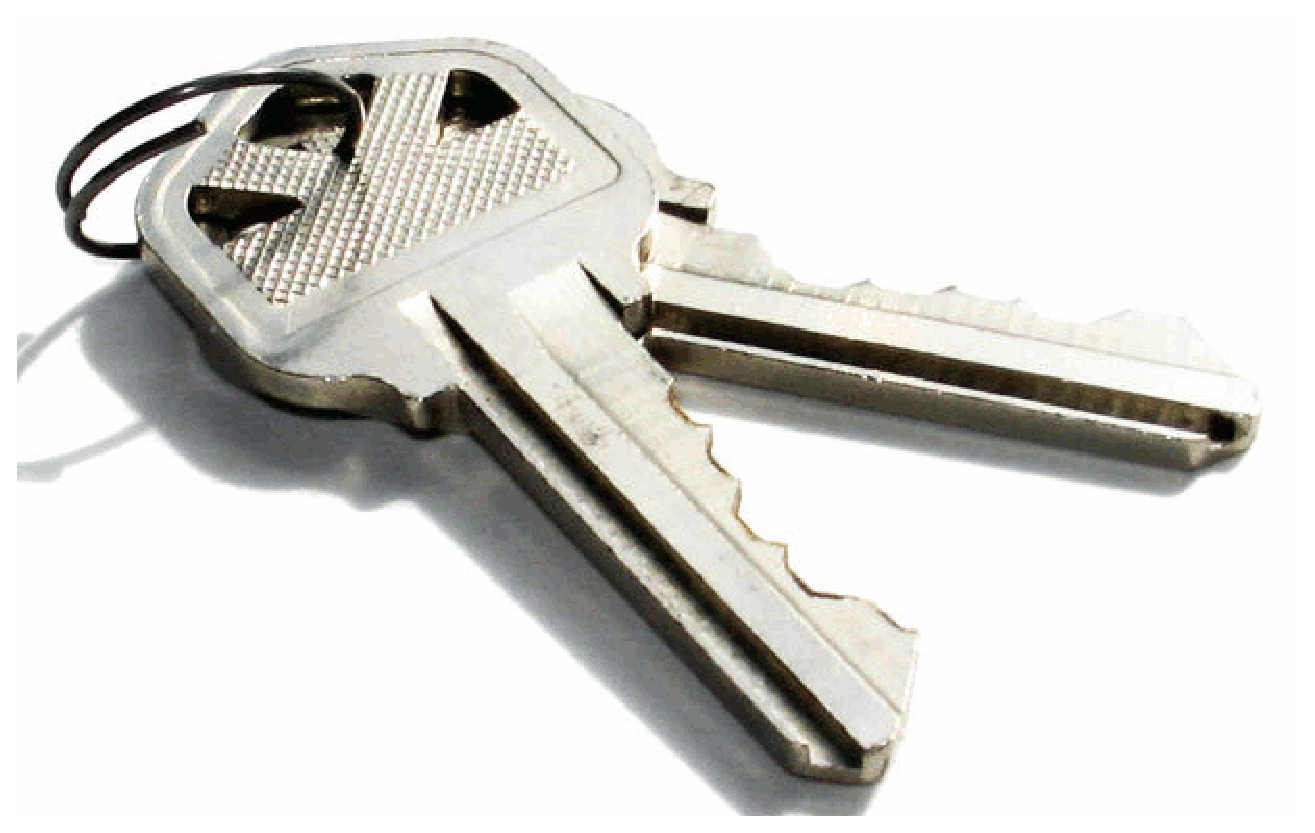
\includegraphics[width=5cm]{keys.eps}
    \end{minipage}
    \begin{minipage}{8cm}
      \large{
        POM2 presents a 10 dimensional hypothesis space. To find the critical factors, POM2 uses the KEYS range subset selector. KEYS uses Bayesian contrast set learning to find the single range that most selects for the preferred outcomes. Subsequent iterations of KEYS constrains the simulator to 

      }
    \end{minipage}
    \large{
always include that range. The smallest subset of selected ranges that most improve the final output is the {\em model treatment}.
    }
    \vspace{-0.5em}
\end{kasten}

\begin{kasten}
    \section*{ \hspace{0.1cm} {\color{red} \underline{WHAT WE FOUND}}}
    \vspace{-0.5em}
    \large{
      \begin{minipage}{4.5cm}
          \begin{center}
            {\small{
            Low dynamism: $\sigma=0, \lambda=0$
            
            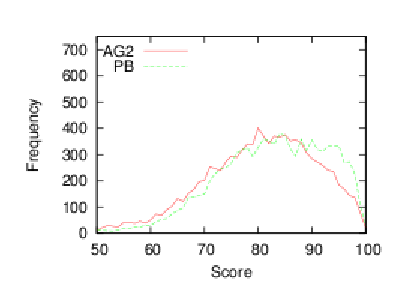
\includegraphics[width=4.5cm]{fr-v-sc-msvl.eps}
            
            Medium dynamism: $\sigma=0.15, \lambda=0.015$
            
            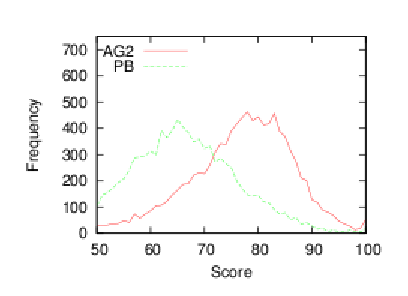
\includegraphics[width=4.5cm]{fr-v-sc-msmi.eps}
            
            High dynamism: $\sigma=2, \lambda=0.2$
            
            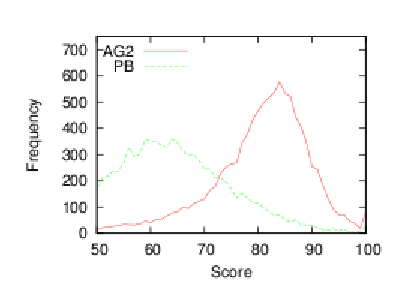
\includegraphics[width=4.5cm]{fr-v-sc-msvh.eps}
            }}
          \end{center}
      \end{minipage}
      \begin{minipage}{8.5cm}
        We ran KEYS 1000 times for each combination of {very low, medium, very high} dynamism and {plan-based, agile 2} prioritization policy. The findings are summarized in \S{RESULTS}. Several majority case effects deserve note:
        \vspace{-0.8em}
        \begin{verysmallitem}
        \item Criticality Modifier: Never chosen in more than $1\%$ of the cases.
        \item Initial Known$/$Inter-Dependency: Never chosen in $>50\%$ of the runs.
        \item Team Size: Never $<5$ team members.
        \item For Agile 2:
          \vspace{-0.7em}
          \begin{verysmallitem}
          \item Size: The smallest size was chosen in $72\%-100\%$ of the runs.
          \item Culture: The upper bins were chosen in $72\%-80\%$ of the runs where dynamism was a factor.
          \item Team Size: Should be 5 - 17 for medium and very high dynamism.
          \end{verysmallitem}
        \end{verysmallitem}

\vspace{-0.8em}
The 1000 runs of KEYS shows that many
results are very similar (e.g. all the Agile 2
          results offer nearly the same pattern). 
KEYS shows that there are two major divisions of 
its 10-dimensional space: very high criticality 
and very small team size. We ran 10,000 
simulations in the union of these two divisions
      \end{minipage}
    }

 (shown above). The median score of Agile 
2 is shows stability under changing dynamism, while 
the median score of Plan-Based falls  as dynamism increases. We see that the median score of Agile 2 is equal to or greater than the median score of Plan-Based development.

    \vspace{3mm}
    We conclude that in the general case, Agile 2 out performs Plan-Based development. Only rarely does Plan-Based out perform Agile 2.
    \vspace{-0.1em}
\end{kasten}

\begin{kasten}
    \section*{ \hspace{0.1cm} {\color{red} \underline{FOR MORE INFORMATION}}}
    \vspace{-0.5em}
    \normalsize{
      Bryan Lemon (\url{bryan@bryanlemon.com})\\
      Tim Menzies Ph.D. (\url{tim@menzies.us})\\
      %Justin Price (\url{justin.n.price@gmail.com})\\
      Joseph D'Alessandro (\url{jdalessa57@gmail.com})
    }
    \vspace{-0.5em}
\end{kasten}

\begin{kasten}
    \section*{ \hspace{0.1cm} {\color{red} \underline{References}}}
    \vspace{-0.5em}
    \normalsize{
      \begin{enumerate}
      \item J. Eisenstein and R. Davis. Visual and linguistic information in gesture classification. In ICMI, pages 113-120, 2004.
      \item R. J. Larsen and M. L. Marx. An Introduction to Mathematical Statistics and Its Applications, Third Edition. Prentice Hall, 2001.
      \item I. H. Witten and E. Frank. Data Mining: Practical Machine Learning Tools and Techniques with Java Implementations. Morgan Kaufmann, 1999.
      \end{enumerate}
    }
\end{kasten}
